\usepackage[utf8]{inputenc}
\documentclass[11pt]{article}
\usepackage{makeidx}
\usepackage{multirow}
\usepackage{multicol}
\usepackage[dvipsnames,svgnames,table]{xcolor}
\usepackage{graphicx}
\usepackage{epstopdf}
\usepackage{ulem}
\usepackage{hyperref}
\usepackage{amsmath}
\usepackage{amssymb}
\author{Bongani Tshela}
\title{}
\usepackage[paperwidth=595pt,paperheight=841pt,top=72pt,right=72pt,bottom=72pt,left=72pt]{geometry}

\makeatletter
	\newenvironment{indentation}[3]%
	{\par\setlength{\parindent}{#3}
	\setlength{\leftmargin}{#1}       \setlength{\rightmargin}{#2}%
	\advance\linewidth -\leftmargin       \advance\linewidth -\rightmargin%
	\advance\@totalleftmargin\leftmargin  \@setpar{{\@@par}}%
	\parshape 1\@totalleftmargin \linewidth\ignorespaces}{\par}%
\makeatother 

\title{External Interface Requirements}
\author{Bongani Tshela 14134790 }
\date{February 2017}

\begin{document}

\maketitle

This section provides a detailed description of all inputs into and outputs from
the system. It also gives a description of the hardware, software and
communication interfaces and provides basic prototypes of the user interface.

\section{User Interface}

{\raggedright
When users open the app, they will find a log-in page where they can enter they're log-in details if they're not first time users. First time users will have to click the register link found on the log in page to register as users of the app or if a user does not want to register, they can continue as guests. Users must note that the privileges of registered will not be the same as those of guests (explained below). 
}

{\raggedright
\uline{Guest Users:}}

{\raggedright
The app will cater for guest users and registered users. Guest users will not have to log in (will use the app as guests). However, when one logs in as a guest, no information about the user will be stored in the database and they will have access to information that is not registered users sensitive (e.g adverts). The guest users will only be able to use the navigation.
}

{\raggedright

}

{\raggedleft
\uline{Registered users:}}

{\raggedright
Registered users will find an extra module(page) where they will be able to add they're favourite events or buildings on campus. They will also be able to import they're timetables after which the app will notify them classes.
}

{\raggedright
\uline{Navigation page:}}

The app will find the users current location (using GPS/network provider info/WI-FI signals). At the navigation page, users will find a single form on which the users will have to submit/enter the desired location.(see picture below for example)

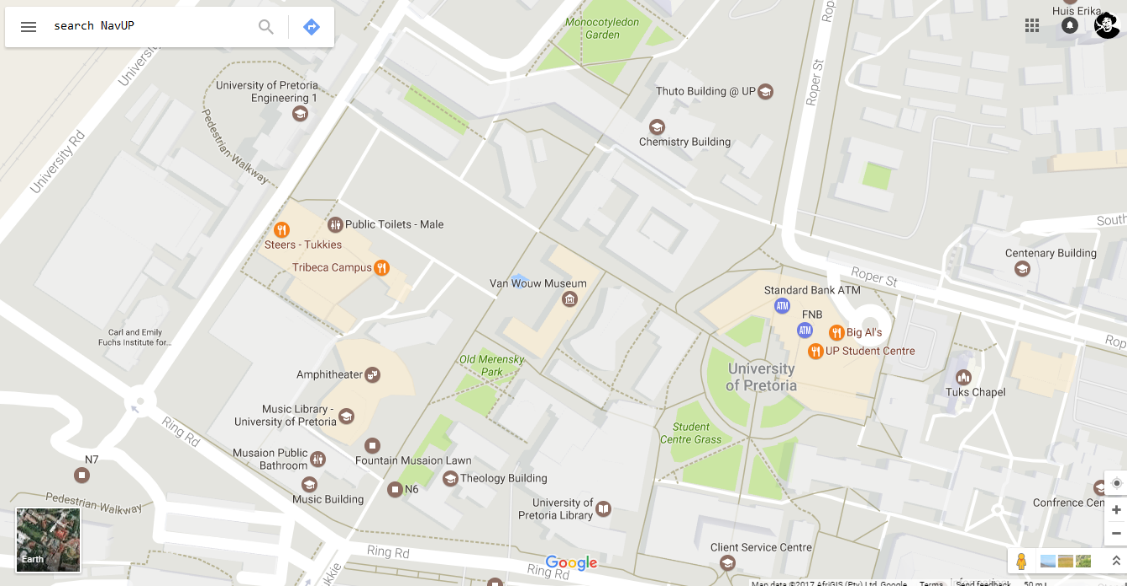
\includegraphics{1.png}

After users have entered the desired location, the app will locate and navigate them to that location. 



\section{Hardware Interface}
{\raggedright
Operation systems or platforms supported: Android, IOS and browsers that support
HTML, CSS, Java-Script (and other web-development and scripting languages). The
NavUP app will depend on the UP Wi-Fi for buildings to be located and devices
using the NavUP app must have Wi-Fi sensors.
The app will also support all types of devices that run the platforms IOS and Android(mobile phones, tablets, phablets). The devices accelerometer can be used to measure how fast or where the person is walking while in-app.
}

\section{Software Interface}
{\raggedright
The app is to be developed for Android, IOS and Web. Android studio will be used
to develop for android (The API Android.location will be used amongst others),
Xcode will id used to develop for ISO and web-development and scripting languages
will be used for the Web app part.
}

{\raggedright

\uline{Software needed or to be implemented:}
}

{\raggedright
Database of users information (SQL+ or MongoDB)
}

{\raggedright
Data structures to store buildings, access points, routs and shortest paths.
}

{\raggedright
Real time data analysis and data streaming tools
}

\section{Communication Interface}
{\raggedright
When the desired location is entered, the coordinates will be sent to the
back-end software/data structure for the app to locate then give directions. The
NavUP app may have a web based server, which will be created using PHP. The
server will retrieve the needed information from the database/data structure. The
HTTP server will use a push protocol to push notifications of updates onto the
user's applications. The Wi-Fi sign on the mobile device that will give indication of signal strength and connectivity.The Communications Interface handles requests to and from the Wi-Fi and application server that will give the user the experience and output needed.Furthermore, whenever a user opens the NavUP app from their
phone, a pull protocol will be used to retrieve and sync the latest updates from
the server.
}


\end{document}
